\section{Overview}
% Researchers universally assume that participants use the input they receive (i.e., the value of each option) to make a choice.
A large body of decision-making research has shown that choice can systematically depend on context. In decision-making experiments, researchers present participants with a finite set of options on each trial and ask them to select a single option based on either an internal (e.g., most preferable) or external (e.g., largest shape) criterion. Decision-making research spans multiple fields, including psychology, neuroscience, economics, marketing, and political science. In economics, for example, researchers have developed models based on the idea that people make choices to maximize their utility but are subject to resource constraints and noisy preferences. In psychology and marketing, however, decision-making researchers have identified a set of phenomena that violate assumptions of certain models of choice, by showing that choices can vary with the \textit{choice set}, or the menu of available options. This class of phenomena is known as \textit{context effects}.

% Context effects are interesting to decision-making researchers because they violate properties exhibited by large classes of choice models, such as Independence of Irrelevant Alternatives (IIA) \parencite{ray1973independence} and regularity \parencite{mackay1995probabilistic,marley1989random}. IIA states that the likelihood of selecting one option over another is invariant of other options available. Regularity states that the probability an option is chosen cannot increase upon the addition of new options to a choice set. IIA and regularity are also properties of Luce's Choice Axiom, a highly influential model of stochastic choice \parencite{luceChoiceAxiomTwenty1977a, luce1959individual}. 

One notable context effect, the attraction effect, occurs when the choice share of a \textit{target} option increases upon the inclusion of a similar but inferior \textit{decoy} option \parencite{huberAddingAsymmetricallyDominated1982d}. Another finding, the repulsion effect, occurs when a decoy boosts the choice share of the dissimilar \textit{competitor} option rather than the target \parencite{simonson2014vices}.  

Context effects, originally studied in preferential choice, have been recently demonstrated in perceptual choice \parencite{trueblood2013not,spektorWhenGoodLooks2018b,liaoInfluenceDistanceDecoy2021,spektorRepulsionEffectPreferential2022,yearsleyContextEffectsSimilarity2022,truebloodPhantomDecoyEffect2017c, turnerCompetingTheoriesMultialternative2018a, evansImpactPresentationOrder2021}. The fact that context effects can appear in perceptual choice is theoretically interesting because it suggests that context effects are a theoretical primitive rather than simply a feature of high-level consumer choice \parencite{trueblood2013not}. 

This dissertation explores various forms of context dependence in both perceptual and preferential choice. Recent work has demonstrated inconsistency in context effects, particularly in perceptual choice. This dissertation uses behavioral experiments and statistical modeling in an attempt to reconcile these inconsistencies. The goal of this dissertation is to further understand why these effects - specifically the attraction and repulsion effects - occur in both perceptual and preferential choice by employing well-studied statistical models from the psychology literature.

This dissertation is structured as follows. Chapter 2, develops and tests a statistical (Thurstonian) model of choice and applies it to perceptual choice. In Experiment 1, it is shown that the types of stimuli used in perceptual choice context effects experiments are easily confusable and vary systematically with theoretically relevant properties of the stimuli. In Experiment 2, the results of a high-powered psychophysics experiment show that the repulsion effect, but not the attraction effect, is naturally predicted by the Thurstonian model. Chapter 3 further tests the Thurstonian model by applying it to best-worst choice. Chapter 4 generalizes the paradigm and the Thurstonian model to preferential choice. Finally, Chapter 5 uses a perceptual choice experiment to show that stimulus comparability affects choice, even when the decoy is equally similar to both focal options. Chapter 6 summarizes the findings of the dissertation, their implications, and discuss future directions for research in this domain. 

Below, the attraction and repulsion effects are introduced, and the empirical and theoretical literaure is reviewed.

\section{The Attraction Effect}
This section formally defines the attraction effect. Let $A$, $B$, $D_{A}$, and $D_{B}$ be discrete choice options, $[]$ denote the options in a choice set, and $P(A|[A,B])$ denote the probability of choosing option $A$ from a set consisting of $A$ and $B$, for example. See Figure~\ref{fig:fig_opts} (left panel), which shows a graphical configuration of the options. These options vary on two dimensions (or attributes), where higher values of an attribute are always preferred. The dimensions are named generically to emphasize the generality of the attraction effect.

In Figure~\ref{fig:att_stim}, options $A$ and $B$ trade off on attributes. $A$ is high on dimension 2 but low on dimension 1, while $B$ is high on dimension 1 but low on dimension 2. A decision-maker who assigns equal importance to both dimensions should be indifferent between both options when presented with choice set $[A,B]$\footnote{The attraction effect does not require the assumption of equal dimension weighting, but it is included here to simplify the example.}. Now, however, consider option $D_{A}$, which is inferior to $A$ and $B$, but more similar to $A$ than to $B$. In decision-making terminology, $D_{A}$ is \textit{asymmetrically dominated} by $A$. $D_{A}$, the \textit{decoy} option, is dominated by $A$, so no rational agent who perceives this dominance relationship should intentionally select the $D_{A}$ over $A$. Similarly, $D_{B}$ is inferior to both $A$ and $B$ but more similar to $B$. The attraction effect is the finding that the relative choice for $A$ over $B$ is greater given set ${A,B,D_{A}}$ then given set $A,B,D_{B}$. 

In the context effects literature, it is common to refer to the similar, dominated option as the \textit{decoy}, the similar dominating option as the \textit{target}, and the dissimilar dominating option as the \textit{competitor}. For example, in the choice set $[A,B,D_{A}]$, $A$ is the target, $B$ is the competitor, and $D_{A}$ is the decoy. This terminology will be adopted throughout this dissertation.
% % \footnote{This is the weak version of the attraction effect. A strong version requires the ordering of P(A) and P(B) to change with choice set. See \textcite{davis2023illustrated} for a discussion of similar issues.}\parencite{huberAddingAsymmetricallyDominated1982d}. 

\begin{figure}
   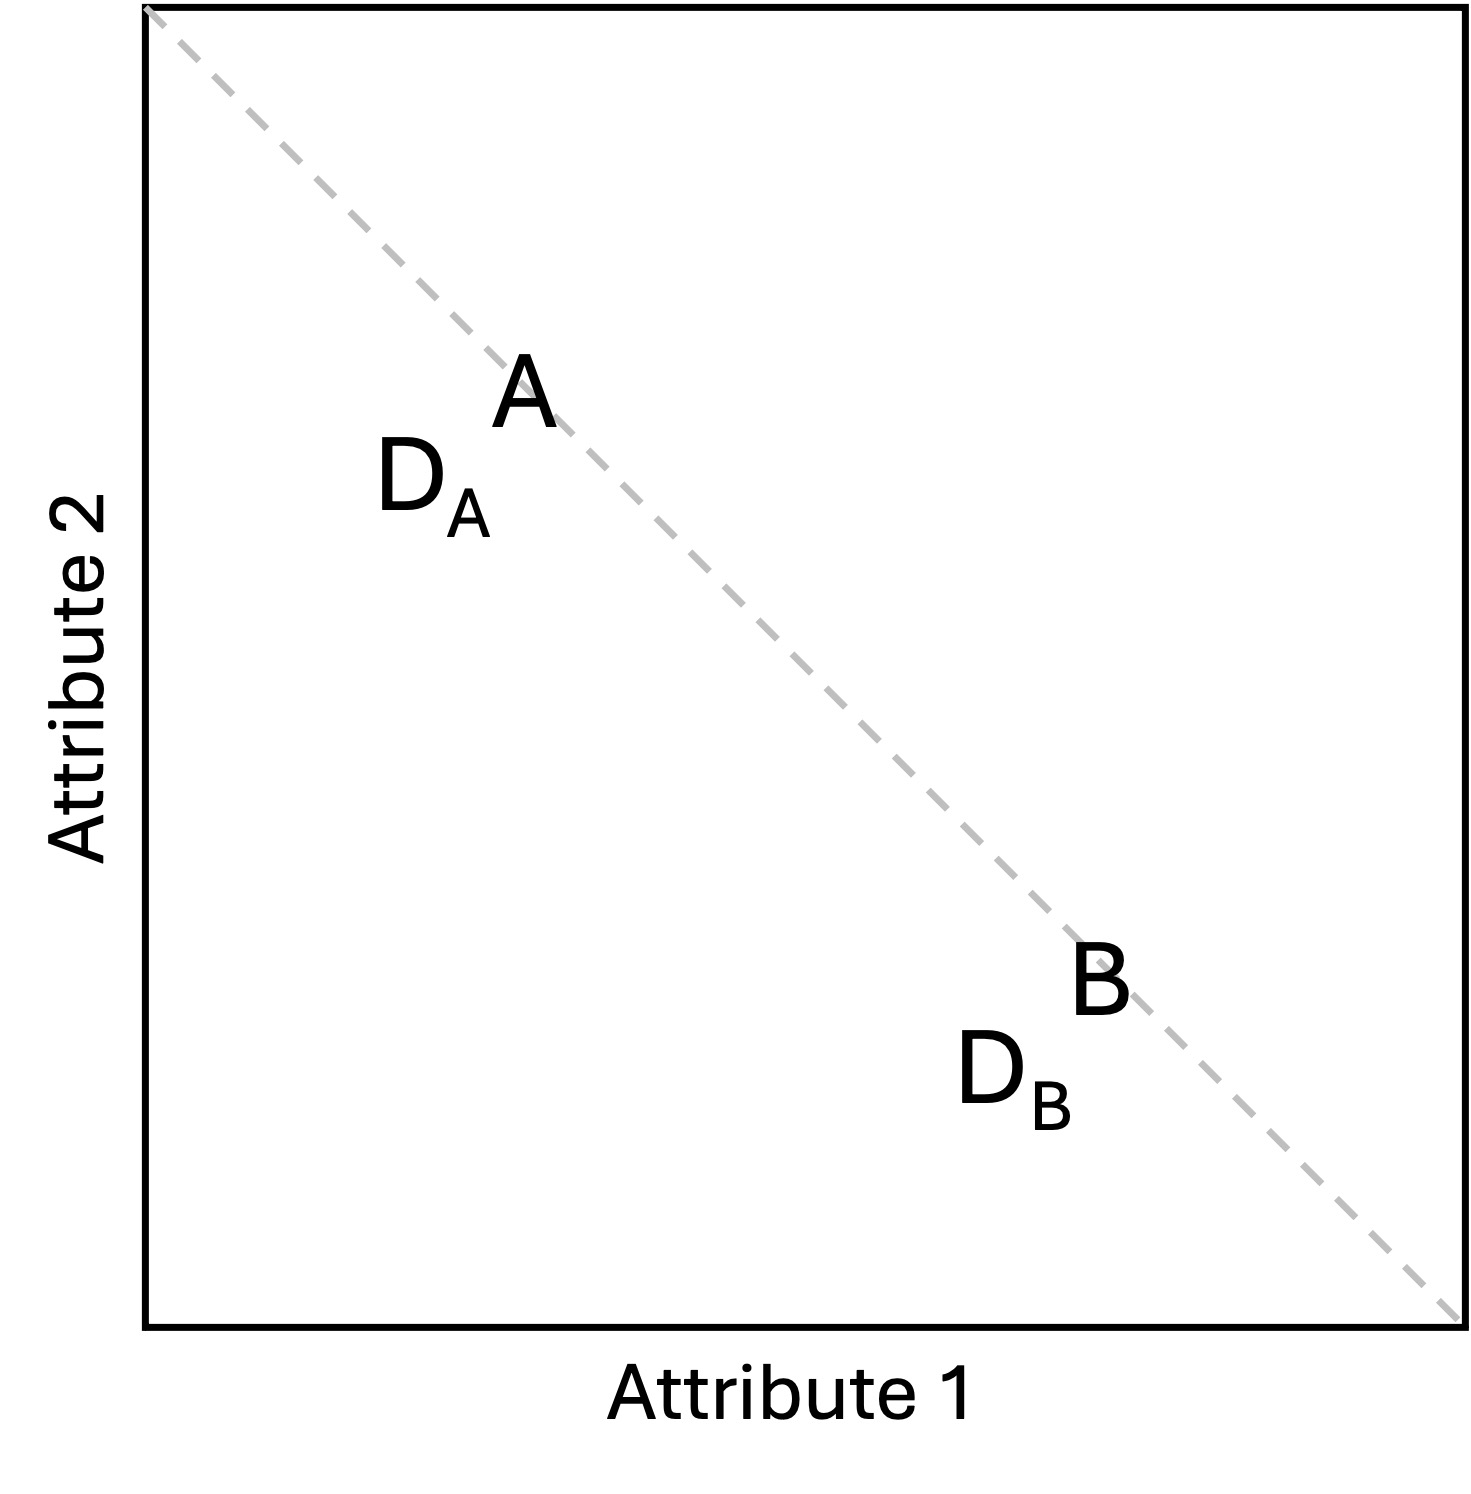
\includegraphics[width=\linewidth]{figures/att_stim.jpg}
   \caption{A graphical depiction of choice options in the attraction/repulsion effect. Attributes are named generically. The diagonal shows the line of indifference, where all options that fall on the line are assumed to be equally valuable (assuming additive utility and equally weighted dimensions).}
   \label{fig:att_stim}
\end{figure}

The attraction effect was first demonstrated by \textcite{huberAddingAsymmetricallyDominated1982d}, who tested participants with sets of choice options, using products such as cars, beers, and TV sets. Participants first completed hypothetical choice tasks where they chose their most preferred option from ternary choice sets, each containing a target, competitor, and decoy option. Participants then returned two weeks later to choose from the same choice sets but with the decoy removed from all trials. Participants chose the target at a higher proportion when the decoy was present than when it was absent. The results of \textcite{huberAddingAsymmetricallyDominated1982d} violate the regularity principle, which states that the choice proportion for a particular option cannot increase when more options are added to the choice set \parencite{mackay1995probabilistic,marley1989random}.

According to regularity, the following inequality should hold:

\begin{equation}
  P(A|[A,B])\geq P(A|[A,B,D_{A}])
  \label{eqn:reg_att}
\end{equation}

Thus, the results demonstrated by \textcite{huberAddingAsymmetricallyDominated1982d}, where $P(A|[A,B,D_{A}])\geq P(A|[A,B])$, violates regularity. \textcite{huberAddingAsymmetricallyDominated1982d} referred to this finding as the asymmetric dominance effect because $D_{A}$ (for example), is necessarily dominated by $A$ but not $B$. $B$ only dominates $A$ assuming Attribute 1 is at least as important as attribute 2. This dissertation will generally use the attraction effect, but the term asymmetric dominance is used where appropriate in reviewing the literature.

The attraction effect also violates the \textit{Independence of Irrelevant Alternatives}(IIA) principle. IIA states that the relative likelihood of choosing a particular option over another is invariant of the choice set \parencite{ray1973independence}. 

Written in the context of the above example, IIA requires the follow equality to hold\footnote{This is often referred to as the constant ratio rule.}: 
\begin{equation}
  \frac{P(A|[A,B])}{P(B|[A,B])}=\frac{P(A|[A,B,D_{A}])}{P(B|[A,B,D_{A}])}
  \label{eqn:iia_att}
\end{equation}

However, in the attraction effect, this equality is violated:
\begin{equation}
  \frac{P(A|[A,B,D_{A}])}{P(B|[A,B,D_{A}])}>\frac{P(A|[A,B])}{P(B|[A,B])}
  \label{eqn:iia_att1}
\end{equation}

The attraction effect is often demonstrated by a ternary-ternary comparison, where participants choose from two choice sets each containing a target, competitor, and decoy option (e.g., $[A,B,D_{A}]$ and  $[A,B,D_{B}]$ in Figure~\ref{fig:att_stim}). In the ternary-ternary form of the attraction effect, participants are more likely to choose $A$ given $[A,B,D_{A}]$ than given $[A,B,D_{B}]$, and they are also more likely to choose $B$ given $[A,B,D_{B}]$ than given $[A,B,D_{A}]$. This effect can be written using the following inequality, which also violates IIA:

\begin{equation}
  \frac{P(A|[A,B,D_{A}])}{P(B|[A,B,D_{A}])}>\frac{P(A|[A,B,D_{B}])}{P(B|[A,B,D_{B}])}
  \label{eqn:iia_att2}
\end{equation}

Thus, IIA is violated by the attraction effect in this ternary-ternary example. Throughout this dissertation, results will be presented by collapsing over choice set and presenting the proportion of target, competitor, and decoy choices.

Since the initial work of \textcite{huberAddingAsymmetricallyDominated1982d}, a large body of research has developed around the attraction effect, both basic and applied. \textcite{doyleRobustnessAsymmetricallyDominated1999} demonstrated both the attraction effect and a related effect, the phantom decoy effect\footnote{A phantom decoy is a decoy which is bot similar to and superior to the target but which made unavailable at the time of choice, but nonetheless increases target choice \parencite{pratkanisBriefHistoryResearch1992b}.} in real-world supermarket purchases. \textcite{van2021attract} showed that the attraction effect can be used to induce people to choose healthier food items. \textcite{slaughterDecoyEffectsAttributelevel1999b} showed that the attraction effect can be found even without the explicit attribute descriptions commonly used in laboratory experiments, when participants must infer option attributes. 

\textcite{o1995attraction} demonstrated the attraction effect in political choice. They presented participants with actual Illinois state senate candidates described by numerical $0-100$ ratings on various policy questions (e.g., 55 on tax policy, 75 on education), and showed that the inclusion of an asymmetrically dominated decoy candidate increased participants' stated willingness to vote for the dominating candidate. In a second study, they had participants rate candidates for the 1992 presidential election (Clinton, Bush, Perot) on a seven-point scale for two policy issues (defense and health). \textcite{o1995attraction} showed that candidates whose ratings, when plotted in a two-dimensional space, created an asymmetric dominance structure, were more likely to vote for the dominating candidate than voters whose space did not form such a structure. \textcite{schwartz1999more} demonstrated the attraction effect in physicians' decisions for medications treating various ailments (e.g., depression, sinusitis), where physicians were more likely to choose a medication if a similar, but inferior decoy was present. For example, when a decoy with identical efficacy but greater likelihood of side effects (when compared to a target option) was included, physicians chose the target more often.

\textcite{cataldoComparisonProcessAccount2019b} showed that, in preferential choice, context effects can be reversed or eliminated simply by altering stimulus presentation format. For example, they showed that if participants can easily compare pairs of options (e.g., target and decoy) on each dimension, the attraction effect occurs quite strongly, but without this ease of comparison the attraction effect becomes neglible. They argued that these results suggest the importance of the comparison process in generating context effects. \textcite{hasan2025registered} failed to replicate this effect, albeit with different decoys than those of \textcite{cataldoComparisonProcessAccount2019b}. 

% \textcite{changWhichCompromiseOption2008} also varied option display, in either a by-alternative format, where option names are listed as columns while attribute values are listed as rows, or a by-attribute format, where option attributes are columns while option names are rows. The former display makes it more difficult to compare options on a single attribute, while the latter makes it easier. They found that listing options by-attribute increased the choice share of the compromise option, relative to a by-alternative display. 

\textcite{hayes2024attribute} manipulated attribute commensurability in a context effects experiment. When two dimensions are commensurable, they vary on a common unit (e.g., user ratings from 0-10), while incommensurable units exist on incomparable units (e.g., RAM and CPU speed in laptops). They found that when dimensions are commensurable, the attraction effect vanishes, while it still exists strongly when dimensions are incommensurable. This suggests that the attraction effect occurs more strongly when the representation of options encourages between-option comparisons on a single attribute.

Other researchers have demonstrated related context effects. \textcite{tverskyEliminationAspectsTheory1972} demonstrated that a similar, but not necessarily inferior, option can decrease choice for a focal option. For example, an option closer to $A$ than to $B$ on the diagonal indifference line in Figure~\ref{fig:att_stim} can cause a decrease in the choice proportion for $A$. This is known as the \textit{similarity effect}. \textcite{simonsonChoiceBasedReasons1989b} demonstrated the compromise effect, where the placement of an intermediate option between two extremes on a diagonal decreases choice for the extremes. 


Theoretically, the attraction effect is interesting to decision-making researchers because, in violating IIA and regularity, the attraction effect is not predicted by many classical models of choice. Luce's Choice Model \parencite{luce1959individual}, for example, is a well-known model of choice which states that the probability of choosing option $x$ from set $K$ can be written as:

\begin{equation}
    P(x|K) = \frac{v_{x}}{\sum_{y \in K} v_{y}}
\end{equation}

where $v_{i}$ is a ratio scaled variable indicating the value, or utility, of option $i$. Luce's model is highly influential in psychology and has been used to account for data in areas such as categorization \parencite{nosofskyAttentionSimilarityIdentificationCategorization1986} and identification \parencite{townsend1971theoretical}. However, given that the model satisfies both IIA and regularity, the model cannot predict the attraction effect. 

Traditional models of choice, as used in economics and marketing research \parencite{mcfadden2001economic}, treat the \textit{utility}, or value, of each option as a random variable whose parameters are estimated from choice data. According to these models, on each trial of a decision-making experiment, the participant samples option values from these distributions and deterministically chooses the option with the highest sampled value. Typically, these models are used to estimate the latent utility values for each option and determine the participants' underlying preferences. These models are known as \textit{Random Utility Models} (RUMs). When utilities are assumed to follow a Type 1 Generalized Extreme Value distribution, the logit or softmax model is used \parencite{gensch1979multinomial}. The probit model, another popular model, assumes Gaussian distributed utilities \parencite{mcfadden1980econometric}. Typically, though not necessarily, these models assume independently distributed errors, which typically implies IIA. 

Often, though not necessarily, RUMs assume IIA. This assumption can be relaxed, however. \textcite{paetzUtilityIndependenceIIA2018} showed, via simulations, that the probit model can violate IIA by allowing correlations between alternatives. IIA can also be relaxed by estimating choice set or alternative specific coefficients \parencite{rooderkerk2011incorporating} or allowing correlations between options and/or attributes \parencite{haaijer1998utility}. Without such modifications, RUMs are unable to account for context effects. 

Given the large body of published empirical data and the inability of existing models to explain context effects, researchers then developed mathematical process models that attempt to explain the cognitive processes that lead to context effects. One particularly notable model of context effect is \textcite{roeMultialternativeDecisionField2001a}'s Multialternative Decision Field Theory (MDFT) model. MDFT is noteworthy for being the first model to simultaneously account for the attraction, similarity, and compromise effects using a single set of parameters. MDFT builds on evidence accumulation models, which decsribe the decision-making process as a stochastic evidence accumulation process in continuous time \parencite{ratcliff1978theory}. In consumer choice, evidence is represented by preference for each option. According to MDFT, the valence $\boldsymbol{V}$ of each option at time $t$ is computed as:

% % \textcite{tversky1993context}'s context-dependent advantage (CDA) model extended utility models to include background contrast (effects of other choice sets that remain in the decision maker’s mind) and all pairwise advantages and disadvantages between options, explaining 

\begin{equation}
    \boldsymbol{V}(t)=\boldsymbol{C}\bm{M}_1\boldsymbol{W}_1(t) + \boldsymbol{\epsilon}(t)
    \label{eqn:mdft}
\end{equation}

where $\boldsymbol{C}$ is a (symmetric) contrast matrix defining the comparison process, $\boldsymbol{M}$ is a matrix of attribute values, $\boldsymbol{W}$ is a vector of attention weights (defining which attribute is being attended to), and $\epsilon$ is the random error term. 

The valences are then combined into a preference state vector $\boldsymbol{P}(t)$ and a new state is formed at time $t+1$ by:

\begin{equation}
    \boldsymbol{P}(t+1)=\boldsymbol{SP}(t)+\boldsymbol{V}(t+1)
    \label{eqn:mdft1}
\end{equation}

$\boldsymbol{S}$ is a feedback matrix where the diagonal elements allow memory decay for previous preference states, but the off-diagonal elements allow options in a choice set to influence one another through lateral inhibition. \textcite{roeMultialternativeDecisionField2001a} stated that this influence should be negative and its strength should be a decreasing function of distance in attribute space. They did not specify a form to this function, but \textcite{hotalingTheoreticalDevelopmentsDecision2010} amended the model to specify a Gaussian function for the distance, where the value of $\boldsymbol{S}_{ij}$ is computed as:

\begin{equation}
    \boldsymbol{S}_{ij}=\delta_{ij}-\varphi_{2} \cdot e^{-\varphi_{1} \cdot D^2_{ij}}
    \label{eqn:mdft2}
\end{equation}

where $\delta_{ij}=0$ if $i\neq j$ (indicating lateral inhibition), $D^2_{ij}$ is distance in attribute space between options $i$ and $j$\footnote{\textcite{hotalingTheoreticalDevelopmentsDecision2010} also specify that distance should be weighted differently depending on whether one option dominates another, i.e., the dominance dimension vs. the indifference dimension.}, and the $\varphi$ are free parameters. In MDFT, as in other evidence accumulation models, preferences continue to accumulate until one option reaches an upper threshold, at which point a choice is made and the decision process stops.

MDFT can produce the attraction effect because of the strong connection between target and decoy (e.g., $A$ and $B$ in Figure~\ref{fig:att_stim}), where the mutual negative inhibition cancels (via multiplication) to cause the decoy to boost the preference state for the target, relative to the competitor. \textcite{mohr2017attraction} demonstrated the attraction effect in risky choice and showed that the MDFT can account for decreases in the size of the attraction effect by allowing for stronger weighting of the subjective distance between target and decoy. In other words, the model predicts that as the decoy is further away, psychologically speaking, from the target, choice for the target will decrease.

\textcite{roeMultialternativeDecisionField2001a} noted that if the off-diagonal elements of $\boldsymbol{S}$ are set to $0$, the MDFT reduces to a form of classical Thurstonian choice model, indexed over time. \textcite{thurstone1927law} showed that given binary choice proportions (for example, participants' choices discriminating between two perceptual stimuli), the \textit{psychological} distance between stimuli can be estimated by assuming Gaussian distributions to the underlying psychological scale. Thurstone's model has various forms (referred to as Cases I-V in the original article), each with various assumptions about the parameters of the model, in particular whether the distributions are independent or correlations are allowed. When the Gaussian distributions are independent, Thurstone's model is unable to predict the attraction effect or similar violations of IIA. 

\textcite{berkowitschRigorouslyTestingMultialternative2014b} tested the independent logit and independent probit models against the MDFT. In their experiment participants chose between digital cameras from choice sets designed to elicit context effects. \textcite{berkowitschRigorouslyTestingMultialternative2014b} found that MDFT, but not the logit or probit models, could account for the attraction effect. Independent RUMs, such as the independent logit and independent probit model, assume each option's utility is independently sampled, so these models cannot account for context effects. Furthermore, according to model comparison measures, the majority of participants were best described by MDFT. Participants whose data were best described by MDFT were also more likely to exhibit context effects. 

The MDFT is not the only cognitive process model developed to explain context effects. \textcite{usherLossAversionInhibition2004a}'s Leaky Competing Accumulators (LCA) model offered an alternative explanation of the attraction effect. LCA uses loss aversion, the idea that losses on a dimension are weighted more heavily than gains on a dimension \parencite{tverskyAdvancesProspectTheorya}, to account for the attraction effect via an asymmetric loss function. In LCA, each option in a choice set is a reference point to all other options. LCA explains the attraction effect through loss aversion because preference for the target is hurt by its relatively large subjective distance from both the target decoy. \textcite{truebloodMultialternativeContextEffects2012} demonstrated context effects in an inference tasks, where participants chose the most likely suspect to have committed a crime from a set of three possible suspects, each described by two numerical ratings describing the strength of eyewitness accounts. \textcite{truebloodMultialternativeContextEffects2012} used this result to argue that the loss aversion account, which may be plausible in preferential choice, is an implausible mechanism for non-preferential tasks. \textcite{trueblood2013not} demonstrated the attraction, similarity, and compromise effects in perceptual choice tasks, where participants were told to select the largest rectangle against a set of rectangles varying in height and width. \textcite{trueblood2013not} argued similarly that loss aversion is an implausible mechanism for the attraction effect in a perceptual task. Other researchers have since demonstrated context effects in perceptual tasks \parencite{choplinComparisoninducedDecoyEffects2005b,yearsleyContextEffectsSimilarity2022,liaoInfluenceDistanceDecoy2021,spektorWhenGoodLooks2018b,spektorRepulsionEffectPreferential2022}. 

Indeed, a large class of cognitive models has emerged to explain context effects \parencite{bhatiaAssociationsAccumulationPreference2013b,noguchiMultialternativeDecisionSampling2018a,trueblood2014multiattribute,wollschlager2NaryChoiceTree2012a,bergnerVAMPVotingAgent2019b,spektor2019similarity}. Modern psychological models of context effects often assume an attribute-wise comparison process \parencite{roeMultialternativeDecisionField2001a,trueblood2013not,usherLossAversionInhibition2004a,bhatiaAssociationsAccumulationPreference2013b}. Under this class of models, participants arrive at a decision by comparing pairs of options on a single attribute, where the modeller assumes attribute values are veridical. This assumption is quite reasonable when modeling choices where each attribute is presented separately and discriminability issues are minimal or non-existent. In perceptual choice experiments, however, like those presented by \textcite{trueblood2013not}, these assumptions are likely incorrect. However, the general modeling framework, where inter-stimulus comparison leads to preference, which then leads to choice, is still plausible. 

There are important limitations to the attraction effect. \textcite{frederickLimitsAttraction2014b} argued that consumer choice researchers who study the attraction effect tend to use simple stimuli varying on few attributes which are described by numeric values, but real-world consumer choice relies heavily on perception, often via images and/or verbal descriptions of produccts. They conducted a large series of studies (over 30), attempting to demonstrate the attraction effect with both abstract numeric stimuli or with perceptual consumer choice stimuli (e.g., a TV with a lower price but an accompanying photo demonstrating slightly fuzzy picture quality as a decoy for a similar priced TV with clearly superior picture quality). \textcite{frederickLimitsAttraction2014b} found that very few studies ($2/33$) using perceptual consumer stimuli demonstrated the attraction effect. They argued that the attraction effect is overrepresented in the literature relative to its real world application. \textcite{yangMoreEvidenceChallenging2014} independently conducted a large scale series of studies attempting to demonstrate the attraction effect with similar stimuli and found that only $2/54$ studies using perceptual or verbally described consumer stimuli showed the attraction effect. \textcite{simonson2014vices} acknowledged the results of \textcite{frederickLimitsAttraction2014b} but argued that researchers should consider the factors that do generate the repulsion effect, such as participant attention, and crucially, whether the asymmetric dominance relationship between target and decoy is perceived by the participant. 

\textcite{trendlZeroAttractionEffect2021} also attempted to demonstrate the attraction with non-numerical, naturalistic stimuli. They had participants rate a number of popular movies,with pre-determined similarities based on both overlapping genre and subgenre categories and human similarity ratings gathered from pilot data. The researchers then used these ratings to create sets of target, competitor, and decoy options, tailored to individual particpants, which were then presented to the participants at a later date. Participants were asked to select their favorite movie from each set. The results showed a clear null attraction effect and \textcite{trendlZeroAttractionEffect2021} argued similarly to \textcite{frederickLimitsAttraction2014b} that the attraction effect may not generalize to naturalistic stimuli.

\textcite{fang2024context} argued that to demonstrate context effects, researchers need an adequate understanding of participants' subjective, psychological representation of the stimuli. They asked college basketball fans to plot NCAA men's basketball teams on a 2-dimensional plot, where the dimensions were offensive and defensive ability. From these representations, they created triplets, tailor-made to each participant, with a target, competitor, and decoy option. In a second phase of the task, participants were presented with these triplets and, for each team in the triplet, they estimated the probability that the given team would out-rank the other two at the end of the season\footnote{In NCAA basketball, teams are ranked weekly by coaches and sports journalists, with the last ranking taking place after the NCAA tournament championship game.}. They found the attraction effect, but only when the subjective target-decoy distance (in psychological space) was high; when it was low, they found the repulsion effect, where the competitor was chosen more than the attraction effect.

The repulsion effect is, empirically speaking, a reversal of the attraction effect. It was first demonstrated in a consumer choice experiment reported by \textcite{frederick2008attraction} who showed that in a consumer choice experiment with TVs, the attraction effect could be reversed to a repulsion effect by representing picture quality perceptually rather than with numerical rating. \textcite{frederickLimitsAttraction2014b} also reported a repulsion effect in one of their studies\footnote{The TV study from \textcite{frederick2008attraction} may have been the same study reported in \textcite{frederickLimitsAttraction2014b}.}. 

Though the repulsion effect has been studied far less than the attraction effect, a recent series of papers have revived interest in the effect. \textcite{spektorWhenGoodLooks2018b} demonstrated the repulsion effect using the same perceptual stimuli as \textcite{trueblood2013not} but represented differently on screen\footnote{The details of this study are discussed at length in Chapter 2.}. \textcite{spektorRepulsionEffectPreferential2022} demonstrated the repulsion effect with both perceptual and risky choice stimuli in a format similar to \textcite{spektorWhenGoodLooks2018b}. \textcite{liaoInfluenceDistanceDecoy2021} conducted a perceptual choice (rectangle) experiment, varying the target-decoy distance (in attribute space, TDD). They found a non-monotonic relationship between TDD and the attraction/repulsion effect. In perceptual choice, low and high TDD values produced a repulsion effect while relatively moderate TDD values produced an attraction effect. In an inference task similar to that of \textcite{truebloodMultialternativeContextEffects2012}, \textcite{liaoInfluenceDistanceDecoy2021} found a different non-monotonic relationship between TDD and the attraction effect; low and high TDD values produced an attraction effect while moderate TDD values produced the repulsion effect. \textcite{brendlPreferentialAttractionEffects2023} demonstrated the repulsion effect with consumer choice stimuli, but only when attributes were represented qualitatively; when attributes were represented quantitatively, they found the attraction effect.

There has been relatively little theoretical progress towards explaining the repulsion effect. \textcite{frederick2008attraction} proposed the \textit{tainting hypothesis}, the idea that the decoy sometimes decreases the subjective value of the nearby target, though evidence for the tainting hypothesis is mixed. \textcite{spektorWhenGoodLooks2018b} found that the repulsion effect weakened with TDD, which will be explored more in Chapter 2. The tainting hypothesis is unable to explain the non-monotonic relationship between TDD and attraction/repulsion found by \textcite{liaoInfluenceDistanceDecoy2021}. \textcite{spektorElusivenessContextEffects2021} argued that understanding how people subjectively represent stimuli in decision-making is crucial to understanding the repulsion effect; in particular they argue that attributes are represented less concretely in perceptual decision-making.

There is much progress to be made, empirically and theoretically, in understanding the conditions that produce the attraction and repulsion effects. The existing literature has demonstrated that the attraction effect can be robust, but perhaps only under certain conditions; the results are far less clear with the repulsion effect, where researchers are just beginning to hypothesize mechanisms to generate the effect. 

The goal of this dissertation is to further understand the attraction and repulsion effects and the mechanisms that generate (some forms of) context-dependence in decision-making. This work builds on the literature discussed here but also in Chapter 2, where the repulsion effect is explored in greater depth. 
 

